\documentclass{dense_template}
\newcommand*{\name}{Felipe Alejandro Jiménez Castillo}
\newcommand*{\code}{215671386}
\newcommand*{\school}{Universidad de Guadalajara - CUCEI}
\newcommand*{\course}{Computación Tolerante a Fallas}
\newcommand*{\assignment}{Servicios}
\renewcommand{\contentsname}{Contenido}

\begin{document}
\maketitle
%%%%%%%%%%%%%%%%%%%%
\tableofcontents
\newpage
%%%%%%%%%%%%%%%%%%%%
\section{Introducción}
Los hilos, procesos, demonios y concurrencia son conceptos fundamentales en la programación y la informática que se utilizan para administrar y ejecutar tareas de manera eficiente en sistemas computacionales.

\begin{itemize}
    \item \textbf{Servicio}
    \begin{itemize}
        \item Un servicio en un sistema operativo es un programa o proceso que se ejecuta en segundo plano sin la intervención activa del usuario y proporciona funcionalidades o recursos específicos al sistema operativo o a otras aplicaciones. Estos servicios pueden ser esenciales para el funcionamiento del sistema o pueden ofrecer características adicionales y funciones.
    \end{itemize}
\end{itemize}

%%%%%%%%%%%%%%%%%%%%
\section{Desarrollo}
\subsection{Script (\textit{python})}
El desarrollo de este servicio se basa en dos funcionalidades, aunque la primaria es el script que realiza la obtención de los datos o estados necesario a mostrar. Para ello se busco una forma de buscar la compatibilidad, por lo que python fue el candidato principal debido a su facilidad de obtención y sencilla forma de tratar errores.
El script se basa en una petición a un endpoint con información de la tasa de cambio sobre ciertas monedas, para el caso particular el Dolar y Bitcoin, para, finalmente, lanzar una notificaión que nos muestre dicha información reciente.

\subsection{Servicio (\textit{systemd})}
El segundo paso para completar nuestro objetivo era hacer que dicho script se ejecutara siempre, en cada reinicio de nuestra maquina o en cierto momento dado. Para ello se opto por systemd, el sistema de inicio y administración de servicios de Linux, lo que nos provee de una implementación sencilla y compacta de, directamente, un servicio con reglas de ejecución, momentos para ejecutarse y más, por lo que basto con crear nuestro servicio, indicarle que realizaría y cando lo haría.




 \begin{center}
    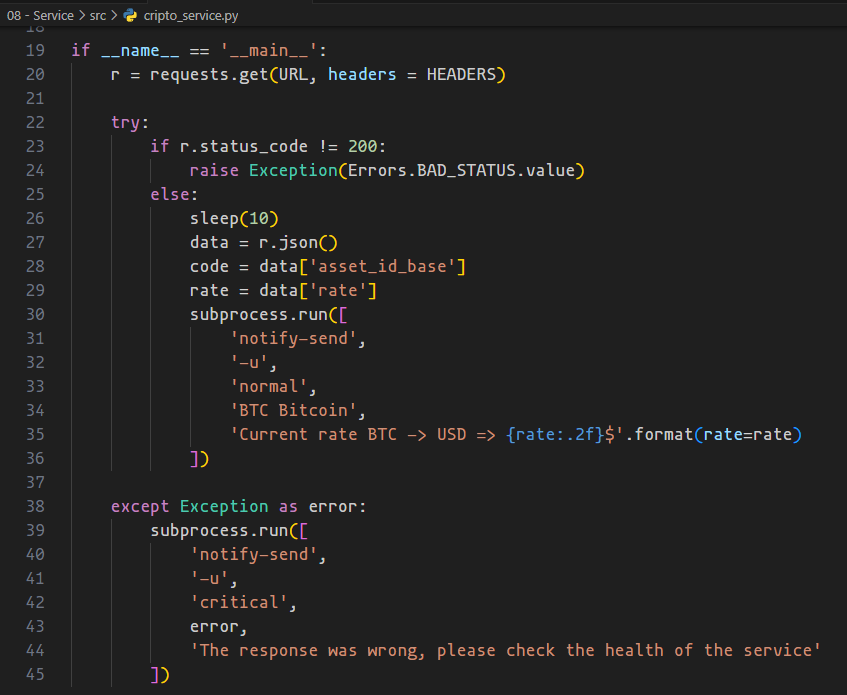
\includegraphics[width=0.6\textwidth]{notifications.png}
    \vspace{1cm}
    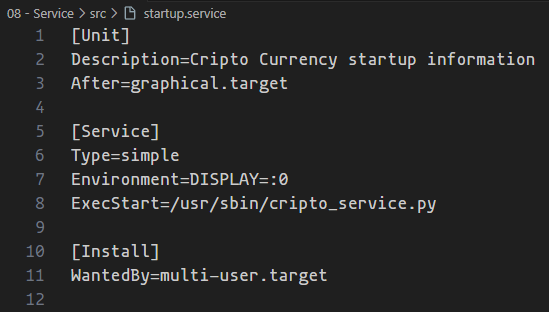
\includegraphics[width=0.6\textwidth]{systemd-service.png}
 \end{center}
%%%%%%%%%%%%%%%%%%%%
\pagebreak
%%%%%%%%%%%%%%%%%%%%
\section{Conclusión}

 Los servicios y procesos en segundo plano son componentes esenciales que trabajan silenciosamente detrás de escena para garantizar el funcionamiento eficiente, confiable y seguro de un sistema operativo. Sin ellos, la experiencia del usuario sería limitada y el sistema sería menos capaz de realizar múltiples tareas y gestionar recursos de manera  efectiva. Su importancia radica en su capacidad para mantener el sistema en funcionamiento y proporcionar una base sólida para que los usuarios y las aplicaciones realicen sus tareas y comunicaciones de manera efectiva.


%%%%%%%%%%%%%%%%%%%%
\pagebreak
%%%%%%%%%%%%%%%%%%%%
\section{Bilbiografia}
\sloppy
\begin{enumerate}
    \item Tanenbaum, A. S. (2004). \textit{Sistemas operativos modernos}. Prentice Hall.
\end{enumerate}
\end{document}

